\section{A terminating ordered normalization}\label{cr:normalization}

A formal leaf now has a nonempty label block $B$ and weight $W_B$. Different live leaves have disjoint blocks. The procedure in this section never tests whether $W_B=0$.

First replace every $\Turn^2$ by $\tau$ and propagate the half-turn through the subtree using \eqref{cr:rotation-rules}. Resolve it on the integral leaves. Reassociate consecutive products into maximal ordered stacks, each with at least two factors. Their factors have the forms
\begin{equation}\label{cr:stack-factors}
              h(B),\qquad \Turn h(B)=R^{W_B},\qquad \Turn(P),
\end{equation}
where $P$ is another maximal stack. The second form is a \emph{direct integral factor}: it is integral at this particular stack, not behind another turn.

Choose a deepest stack with at least two direct integral factors. Slide all those factors to its right end by Lemma~\ref{cr:slide}, then fuse them. The new integral factor carries the union of their blocks and the sum of their weights. Propagate all rotations by \eqref{cr:rotation-rules}, shorten turn chains and flatten adjacent products again. Fix an order for every choice, for example first in the current ordered traversal.

A rotated direct integral remains direct integral; a rotated ordinary leaf remains ordinary; a rotated turned stack remains a turned stack. Consequently this propagation does not hide an integral factor by replacing a rotated arbitrary tangle by the original one. Each fusion decreases the number of live leaves, even if the new sum is zero. Between fusions there are only finitely many turn-shortening and flattening operations, and the propagation visits a finite tree without introducing leaves. The procedure terminates after at most $m-1$ fusions.

\begin{lemma}[The reduced-stack types]\label{cr:reduced-stacks}
When every maximal stack has at most one direct integral factor, every other factor has type $L$ or $A$. A stack with no direct integral has type $A$; a stack with one has type $H$. Any ordered binary resolution of such a stack passes the product table.
\end{lemma}
\begin{proof}
Induct upward from the deepest stacks. Ordinary leaves have type $L$. A child stack has type $A$ or $H$ by induction, so its turn has type $A$ or $L$. At least two $L/A$ factors multiply to $A$. Inserting the single $H$ factor yields $H$, and no intermediate grouping can encounter two $H$ factors. If a stack has collapsed to one factor during fusion, that factor is integral: it results from fusing all the former factors, not from deleting arbitrary subtrees. Suppress this unary stack before applying the induction.
\end{proof}

For the input $C(FG)$ the root is still a product unless all its factors fuse to one integral box. The latter case is the stated elementary output. Otherwise write the normalized maximal root stack with $k\ge2$ factors. If $k\ge3$ and none is integral, expose one $L/A$ factor against the product of the rest, of type $A$. If one is integral, use closed cyclicity to expose it against the other $k-1$ factors, again of type $A$. Both closures pass the table.

When $k=2$, all pairs pass except $LL$. A type-$L$ factor is literally $\Turn U$, where $U$ is either a single integral box or a stack with precisely one direct integral factor. This includes $h(B)=\Turn R^{W_B}$. The failed root therefore has the actual isotopy
\begin{equation}\label{cr:failed-root}
                C((\Turn U)(\Turn V))\simeq C(U\tau V).
\end{equation}
Flattening exposes the one integral from each side, together with $L/A$ factors. Slide and fuse these two integrals, retaining all rotations, and normalize again. This return makes a genuine fusion. Thus the full root procedure terminates too. Zero sums remain named integral boxes; they are not removed in this section.

Each step preserves or unions disjoint label blocks. Fixing the original parities determines the parity of every moved sum and hence every rotation. The entire ordered schedule and the resulting structural expression are therefore fixed on a parity class, even when some sums happen to vanish. This proves the existence and isotopy assertions of Theorem~\ref{cr:ordered}. We next strengthen the bookkeeping by showing that its partition can be chosen independently of parity.

\section{The net blocks before assigning parities}\label{cr:partition}

There is a useful finite graph underlying the normalization. It records tangle operations and turn parity, not a new knot projection. Remove the last closing product and join the output ends of $F$ and $G$. Represent every remaining product by a trivalent vertex. Put a bit in $\{0,1\}$ on each edge recording the number of quarter-turns on it modulo two. A leaf ends at the integral braid $R^{n_i}$, so the turn in $h_i=\Turn R^{n_i}$ contributes one to its leaf-edge bit.

For $m\ge3$ the graph is an unrooted tree with $m$ labelled leaves and internal vertices of valence three. Contract every internal edge with bit zero. This joins associative product regions. The result is a tree of junctions of valence at least three, with bit one on every internal edge. At a junction $v$, call the labels on its bit-zero leaf edges $I_v$. These are exactly its direct integral labels. The partition is
\begin{equation}\label{cr:partition-formula}
 \{I_v:I_v\ne\varnothing\}\ \cup\
 \{\{i\}:\text{the leaf edge at }i\text{ has bit one}\}.
\end{equation}
Every label occurs in exactly one displayed set.

\begin{proposition}[Parity-independent blocks]\label{cr:blocks}
The blocks in \eqref{cr:partition-formula} are exactly the blocks of an ordered normalization by the preceding isotopies. No second union is needed after a junction is suppressed. For $m=2$, equal total leaf bits give the single block $\{1,2\}$, while unequal bits give the two singleton blocks.
\end{proposition}
\begin{proof}
Use Lemma~\ref{cr:expose} to place a chosen junction at the closing sphere, then gather its entire direct integral set. All slides retain the rotations and orders of the attached subtrees. A rotation in \eqref{cr:rotation-rules} preserves every edge's turn parity and every leaf label. Associativity joins vertices across zero-bit edges. Moving a turn across the closing sphere preserves the total turn bit on that unrooted edge. The failed $LL$ root in \eqref{cr:failed-root} has two turns and hence total bit zero: its two product regions already belong to the same contracted junction. Its exposed integrals thus belong to the same prescribed $I_v$.

Fusing $I_v$ to one integral leaf may lower the junction's valence. If the new valence is two, its incidences consist of that integral leaf and one other edge. If the other edge is internal, its bit is one. Suppressing the junction sends the integral leaf through this turn, and its neighbor receives an ordinary leaf. The neighbor's valence is unchanged, and it receives no new direct integral label. Thus suppression cannot create a further union. If two such two-valent junctions meet across an internal turn edge, suppressing either yields a two-leaf mixed closure with one total turn. If the other incidence is already an ordinary leaf, this is the same mixed closure. A one-valent junction has only its fused integral leaf and, by connectedness, is the whole graph; it gives the elementary closure.

These are all possibilities: before fusion every junction had valence at least three, and only its direct leaves were replaced. There is no unrecorded deletion of another subtree. Performing junction fusions in a fixed order and these suppressions gives a schedule of the physical moves in Sections~\ref{cr:rotations}--\ref{cr:closing}. The surviving junctions pass Lemma~\ref{cr:reduced-stacks}. This realizes exactly \eqref{cr:partition-formula}.

For two leaves there is no junction. Equal bits have total bit zero: with two turns use \eqref{cr:double-turn}, and with none concatenate the braids. Both give $C(R^{n_1+n_2})$. Unequal bits give the strict mixed closure $C(R^{n_1}h_2)$. The rotations act trivially on individual integral leaves. The graph and its blocks depend only on the original syntax; parities choose the subsequent order reversals but do not change a block.
\end{proof}

\begin{figure}[ht]
\centering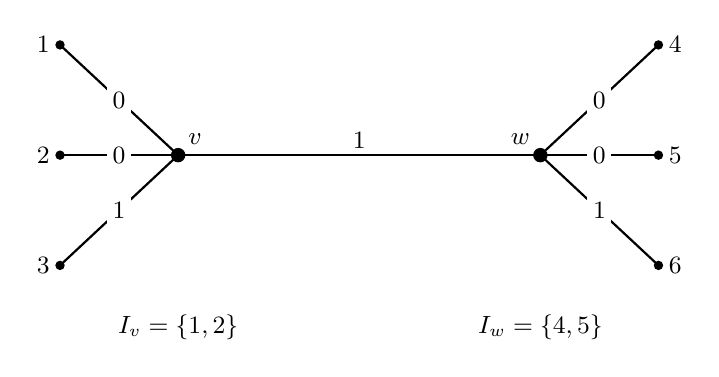
\begin{tikzpicture}[line cap=round,thick,every node/.style={font=\small},
 bit/.style={fill=white,inner sep=2pt}]
\coordinate (v) at (0,0);\coordinate (w) at (4.6,0);
\draw (v)--node[bit,above] {$1$}(w);
\foreach \name/\x/\y/\b in {1/-1.5/1.4/0,2/-1.5/0/0,3/-1.5/-1.4/1}{
 \draw (v)--node[bit] {$\b$}(\x,\y);
 \fill (\x,\y) circle(1.7pt);\node[left] at(\x,\y){$\name$};}
\foreach \name/\x/\y/\b in {4/6.1/1.4/0,5/6.1/0/0,6/6.1/-1.4/1}{
 \draw(w)--node[bit] {$\b$}(\x,\y);
 \fill(\x,\y)circle(1.7pt);\node[right]at(\x,\y){$\name$};}
\fill(v)circle(2.6pt);\fill(w)circle(2.6pt);
\node[above right]at(v){$v$};\node[above left]at(w){$w$};
\node[below]at(0,-1.9){$I_v=\{1,2\}$};
\node[below]at(4.6,-1.9){$I_w=\{4,5\}$};
\end{tikzpicture}

\caption{The net blocks for \eqref{cr:example}. Each leaf is an integral box; its edge label is the turn bit. The internal edge has bit one, so the two junctions stay separate. The direct leaves at the left junction fuse to $\{1,2\}$ and those at the right to $\{4,5\}$. Leaves $3,6$ are ordinary singleton blocks. These are label unions; no numerical zero test has been made.}\label{cr:net-figure}
\end{figure}

\subsection{An example and a zero wall}

Consider the explicit ordered expression
\begin{equation}\label{cr:example}
 C\bigl(R^{n_1}R^{n_2}h_3\,
                 \Turn(R^{n_4}R^{n_5}h_6)\bigr).
\end{equation}
It is in the original syntax since $R^{n_i}=\Turn h_i$. Put $a=n_1+n_2$ and $b=n_4+n_5$. Adjacent fusion gives
\[
                     C\bigl(R^a h_3\Turn(R^b h_6)\bigr).
\]
The partition is $\{1,2\},\{3\},\{4,5\},\{6\}$. The inner stack has type $HL=H$, its turn has type $L$, and the closing pair can be chosen $HA$. Thus the resulting formal expression is strict even on $a=0$ or $b=0$; the long-filling theorem applies only when its actual four weights are long.

On the wall $a=0$, removing the through identity is an additional evaluated move. The original rotations give
\begin{align*}
 C\bigl(h_3\Turn(R^b h_6)\bigr)
 &\simeq C\bigl(R^{n_3}\tau(R^b h_6)\bigr)\\
 &=C\bigl(R^{n_3}h_6R^b\bigr)
 \simeq C\bigl(R^{n_3+b}h_6\bigr).
\end{align*}
The surviving blocks have changed to $\{3,4,5\},\{6\}$, with $\{1,2\}$ deleted. The reversal $\tau(R^b h_6)=h_6R^b$ and final closed cyclic move are essential. This example explains why the zero-aware reduction needs a different finite partition statement.
